% Options for packages loaded elsewhere
\PassOptionsToPackage{unicode}{hyperref}
\PassOptionsToPackage{hyphens}{url}
%
\documentclass[
]{book}
\title{Học xác suất thống kê qua phần mềm R}
\author{Duc Nguyen}
\date{2022-02-12}

\usepackage{amsmath,amssymb}
\usepackage{lmodern}
\usepackage{iftex}
\ifPDFTeX
  \usepackage[T1]{fontenc}
  \usepackage[utf8]{inputenc}
  \usepackage{textcomp} % provide euro and other symbols
\else % if luatex or xetex
  \usepackage{unicode-math}
  \defaultfontfeatures{Scale=MatchLowercase}
  \defaultfontfeatures[\rmfamily]{Ligatures=TeX,Scale=1}
\fi
% Use upquote if available, for straight quotes in verbatim environments
\IfFileExists{upquote.sty}{\usepackage{upquote}}{}
\IfFileExists{microtype.sty}{% use microtype if available
  \usepackage[]{microtype}
  \UseMicrotypeSet[protrusion]{basicmath} % disable protrusion for tt fonts
}{}
\makeatletter
\@ifundefined{KOMAClassName}{% if non-KOMA class
  \IfFileExists{parskip.sty}{%
    \usepackage{parskip}
  }{% else
    \setlength{\parindent}{0pt}
    \setlength{\parskip}{6pt plus 2pt minus 1pt}}
}{% if KOMA class
  \KOMAoptions{parskip=half}}
\makeatother
\usepackage{xcolor}
\IfFileExists{xurl.sty}{\usepackage{xurl}}{} % add URL line breaks if available
\IfFileExists{bookmark.sty}{\usepackage{bookmark}}{\usepackage{hyperref}}
\hypersetup{
  pdftitle={Học xác suất thống kê qua phần mềm R},
  pdfauthor={Duc Nguyen},
  hidelinks,
  pdfcreator={LaTeX via pandoc}}
\urlstyle{same} % disable monospaced font for URLs
\usepackage{color}
\usepackage{fancyvrb}
\newcommand{\VerbBar}{|}
\newcommand{\VERB}{\Verb[commandchars=\\\{\}]}
\DefineVerbatimEnvironment{Highlighting}{Verbatim}{commandchars=\\\{\}}
% Add ',fontsize=\small' for more characters per line
\usepackage{framed}
\definecolor{shadecolor}{RGB}{248,248,248}
\newenvironment{Shaded}{\begin{snugshade}}{\end{snugshade}}
\newcommand{\AlertTok}[1]{\textcolor[rgb]{0.94,0.16,0.16}{#1}}
\newcommand{\AnnotationTok}[1]{\textcolor[rgb]{0.56,0.35,0.01}{\textbf{\textit{#1}}}}
\newcommand{\AttributeTok}[1]{\textcolor[rgb]{0.77,0.63,0.00}{#1}}
\newcommand{\BaseNTok}[1]{\textcolor[rgb]{0.00,0.00,0.81}{#1}}
\newcommand{\BuiltInTok}[1]{#1}
\newcommand{\CharTok}[1]{\textcolor[rgb]{0.31,0.60,0.02}{#1}}
\newcommand{\CommentTok}[1]{\textcolor[rgb]{0.56,0.35,0.01}{\textit{#1}}}
\newcommand{\CommentVarTok}[1]{\textcolor[rgb]{0.56,0.35,0.01}{\textbf{\textit{#1}}}}
\newcommand{\ConstantTok}[1]{\textcolor[rgb]{0.00,0.00,0.00}{#1}}
\newcommand{\ControlFlowTok}[1]{\textcolor[rgb]{0.13,0.29,0.53}{\textbf{#1}}}
\newcommand{\DataTypeTok}[1]{\textcolor[rgb]{0.13,0.29,0.53}{#1}}
\newcommand{\DecValTok}[1]{\textcolor[rgb]{0.00,0.00,0.81}{#1}}
\newcommand{\DocumentationTok}[1]{\textcolor[rgb]{0.56,0.35,0.01}{\textbf{\textit{#1}}}}
\newcommand{\ErrorTok}[1]{\textcolor[rgb]{0.64,0.00,0.00}{\textbf{#1}}}
\newcommand{\ExtensionTok}[1]{#1}
\newcommand{\FloatTok}[1]{\textcolor[rgb]{0.00,0.00,0.81}{#1}}
\newcommand{\FunctionTok}[1]{\textcolor[rgb]{0.00,0.00,0.00}{#1}}
\newcommand{\ImportTok}[1]{#1}
\newcommand{\InformationTok}[1]{\textcolor[rgb]{0.56,0.35,0.01}{\textbf{\textit{#1}}}}
\newcommand{\KeywordTok}[1]{\textcolor[rgb]{0.13,0.29,0.53}{\textbf{#1}}}
\newcommand{\NormalTok}[1]{#1}
\newcommand{\OperatorTok}[1]{\textcolor[rgb]{0.81,0.36,0.00}{\textbf{#1}}}
\newcommand{\OtherTok}[1]{\textcolor[rgb]{0.56,0.35,0.01}{#1}}
\newcommand{\PreprocessorTok}[1]{\textcolor[rgb]{0.56,0.35,0.01}{\textit{#1}}}
\newcommand{\RegionMarkerTok}[1]{#1}
\newcommand{\SpecialCharTok}[1]{\textcolor[rgb]{0.00,0.00,0.00}{#1}}
\newcommand{\SpecialStringTok}[1]{\textcolor[rgb]{0.31,0.60,0.02}{#1}}
\newcommand{\StringTok}[1]{\textcolor[rgb]{0.31,0.60,0.02}{#1}}
\newcommand{\VariableTok}[1]{\textcolor[rgb]{0.00,0.00,0.00}{#1}}
\newcommand{\VerbatimStringTok}[1]{\textcolor[rgb]{0.31,0.60,0.02}{#1}}
\newcommand{\WarningTok}[1]{\textcolor[rgb]{0.56,0.35,0.01}{\textbf{\textit{#1}}}}
\usepackage{longtable,booktabs,array}
\usepackage{calc} % for calculating minipage widths
% Correct order of tables after \paragraph or \subparagraph
\usepackage{etoolbox}
\makeatletter
\patchcmd\longtable{\par}{\if@noskipsec\mbox{}\fi\par}{}{}
\makeatother
% Allow footnotes in longtable head/foot
\IfFileExists{footnotehyper.sty}{\usepackage{footnotehyper}}{\usepackage{footnote}}
\makesavenoteenv{longtable}
\usepackage{graphicx}
\makeatletter
\def\maxwidth{\ifdim\Gin@nat@width>\linewidth\linewidth\else\Gin@nat@width\fi}
\def\maxheight{\ifdim\Gin@nat@height>\textheight\textheight\else\Gin@nat@height\fi}
\makeatother
% Scale images if necessary, so that they will not overflow the page
% margins by default, and it is still possible to overwrite the defaults
% using explicit options in \includegraphics[width, height, ...]{}
\setkeys{Gin}{width=\maxwidth,height=\maxheight,keepaspectratio}
% Set default figure placement to htbp
\makeatletter
\def\fps@figure{htbp}
\makeatother
\setlength{\emergencystretch}{3em} % prevent overfull lines
\providecommand{\tightlist}{%
  \setlength{\itemsep}{0pt}\setlength{\parskip}{0pt}}
\setcounter{secnumdepth}{5}
\usepackage{booktabs}
\ifLuaTeX
  \usepackage{selnolig}  % disable illegal ligatures
\fi
\usepackage[]{natbib}
\bibliographystyle{plainnat}

\begin{document}
\maketitle

{
\setcounter{tocdepth}{1}
\tableofcontents
}
\hypertarget{stat-learning}{%
\chapter{Stat learning}\label{stat-learning}}

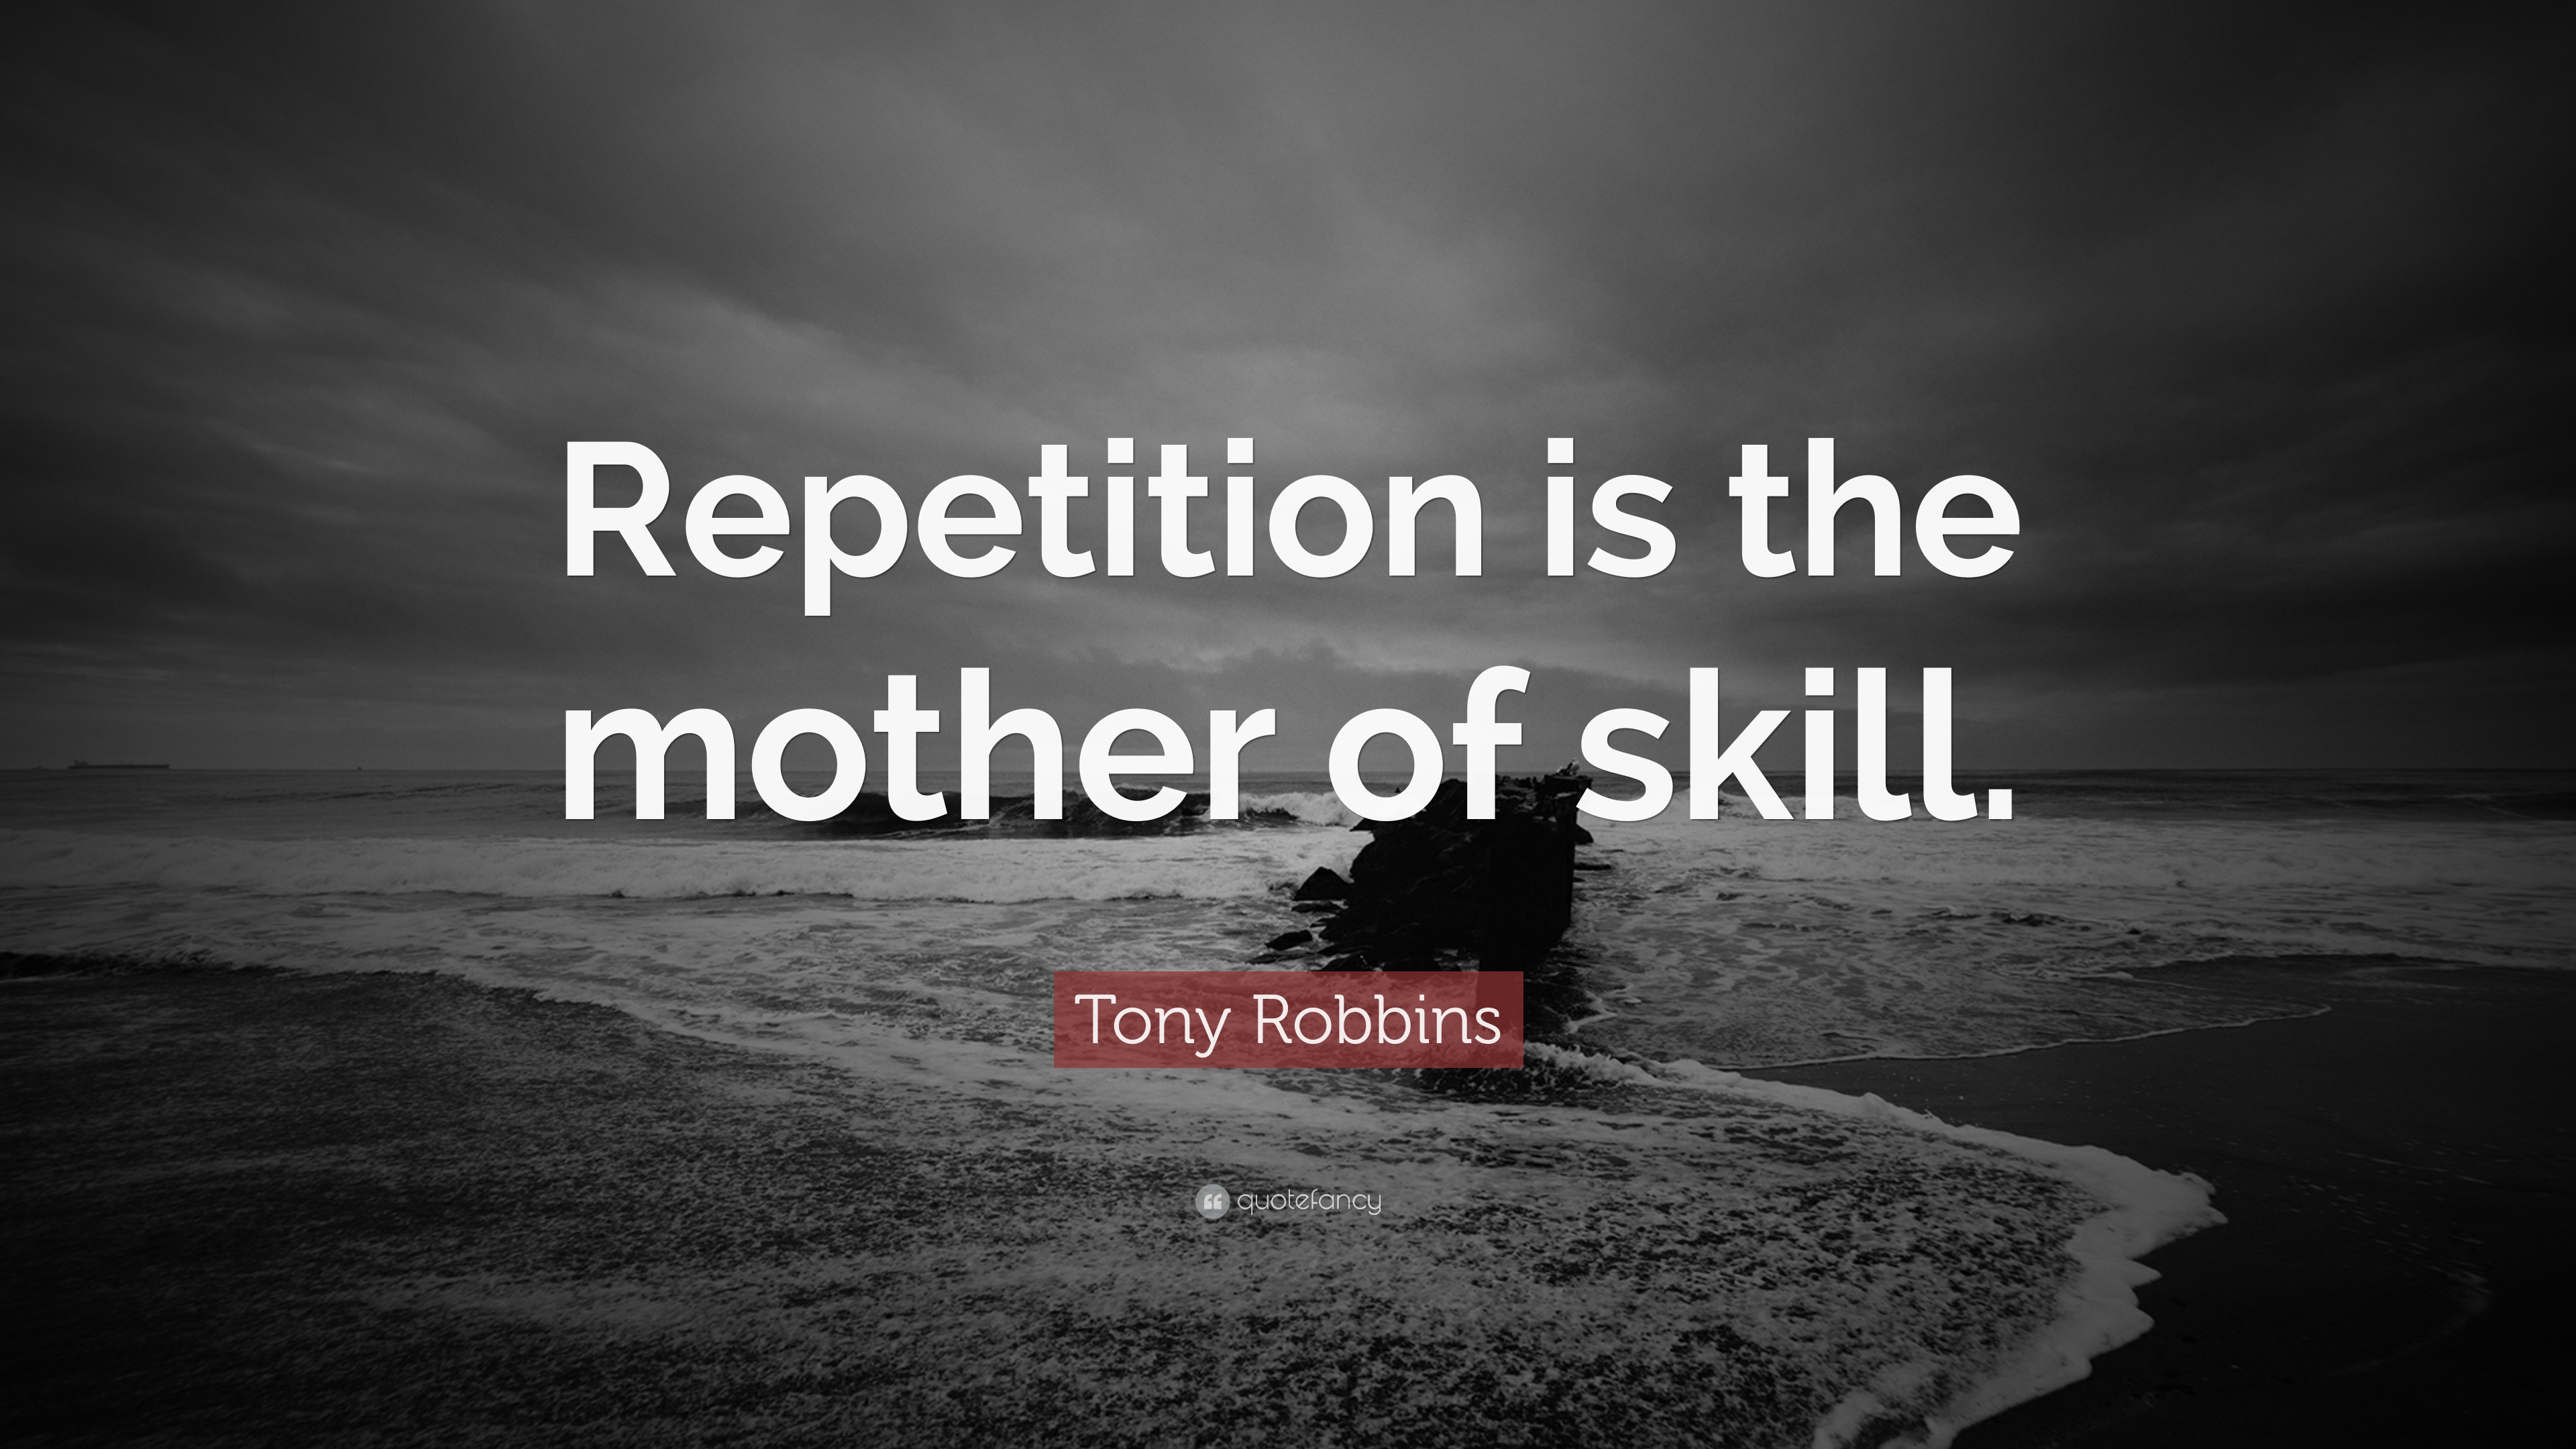
\includegraphics[width=1\textwidth,height=\textheight]{images/Quotefancy-237580-3840x2160.jpg}
Test bookdown for creating better books.
\href{mailto:tanduc307@gmail.com}{\nolinkurl{tanduc307@gmail.com}}

\hypertarget{how-to-use-tools}{%
\chapter{How to use tools}\label{how-to-use-tools}}

\hypertarget{tux1ea1o-thux1b0-mux1ee5c-luxe0m-viux1ec7c}{%
\section{Tạo thư mục làm việc}\label{tux1ea1o-thux1b0-mux1ee5c-luxe0m-viux1ec7c}}

Khi sử dụng Rstudio thì nên tạo thư mục project để toàn bộ files sẽ nằm trong đó.

Cách thực hiện xem ở đây \url{https://alexd106.github.io/intro2R/howto.html\#rstudio_proj-vid}

Lợi thế là trong folder project này, ta có thể tạo các folder con như images, data, tables, \ldots{} để thuận tiện lưu riêng từng loại dữ liệu. {[}hiện tại làm sao để cấu hình cho hình ảnh nó tự động lưu theo từng folder thì chưa biết cách, thấy có package `here' mà không biết cách dùng).

Lưu ý là khi dùng bookdown để render books thì tên của heading là ghi tiếng Anh cho lành, vì nếu ghi tiếng Việt thì nó render bị lỗi unicode.

RStudio Projects from intro 2R on Vimeo.

\hypertarget{chuxe8n-huxecnh-ux1ea3nh}{%
\section{Chèn hình ảnh}\label{chuxe8n-huxecnh-ux1ea3nh}}

Có các cách chèn hình khi sử dụng Rstudio như sau:

• Chuyển qua chế độ Visual rồi insert hình ảnh. Sau đó hình ảnh sẽ được lưu trong folder \_book/images khi render bằng knitr.

• Nếu gõ theo kiểu source code thì dùng đoạn mã sau
\texttt{\textasciigrave{}\textasciigrave{}\textasciigrave{}\ \{r\ echo=TRUE,\ paged.print=FALSE,\ out.width="30\%"\}\ knitr::include\_graphics("images/cover.jpg")\ \textasciigrave{}\textasciigrave{}\textasciigrave{}}

\begin{Shaded}
\begin{Highlighting}[]
\NormalTok{knitr}\SpecialCharTok{::}\FunctionTok{include\_graphics}\NormalTok{(}\StringTok{"images/cover.jpg"}\NormalTok{)}
\end{Highlighting}
\end{Shaded}


\includegraphics[width=0.3\linewidth]{images/cover}

• Nếu copy và paste từ trên Internet thì dùng add-on \texttt{imageclipr} \href{https://github.com/Toniiiio/imageclipr}{\textless https://github.com/Toniiiio/imageclipr\textgreater{}}. Hình ảnh sẽ lưu mặc định trong working directory.

• Nếu copy và paste hình ảnh theo kiểu thủ công thì hình ảnh mặc định sẽ lưu ở \texttt{C:/Users/tandu/AppData/Local/RStudio/tmp/paste-B717C571.png} như vậy thì khi xuất bản online sẽ không thấy. Do đó phải đưa hình ảnh vào trong thư mục project (theo kiểu thủ công) hoặc dùng add-on \texttt{imageclipr} theo kiểu trực tiếp trong Rstudio (nhưng ở dạng Rmarkdown, còn Rmarkdown visual thì bị lỗi).

\hypertarget{chuxe8n-video}{%
\section{Chèn video}\label{chuxe8n-video}}

Sử dụng link này \url{https://video-to-markdown.marcomontalbano.com/} (theo kiểu click vào hình rồi direct qua source để play video)

Hoặc syntax \texttt{{[}!{[}Alternate\ Text{]}(\{image-url\}){]}(\{video-url\}\ "Link\ Title")}

Chèn từ Youtube, sử dụng code embed rồi paste vào.

\texttt{\textless{}iframe\ width="560"\ height="315"\ src="https://www.youtube.com/embed/RLxV3T2b524"\ title="YouTube\ video\ player"\ frameborder="0"\ allow="accelerometer;\ autoplay;\ clipboard-write;\ encrypted-media;\ gyroscope;\ picture-in-picture"\ allowfullscreen\textgreater{}\textless{}/iframe\textgreater{}}

Tuy nhiên video sẽ không tự động resize theo khung cửa sổ

Nên dùng code này để video tự động resize. Chiều rộng và cao 100\% có nghĩa là theo khung cửa sổ chứ không phải theo kích thước gốc của video.

\texttt{\textless{}div\ style="position:relative;padding-bottom:56.25\%;"\textgreater{}\ \ \textless{}iframe\ style="width:100\%;height:100\%;position:absolute;left:0px;top:0px;"\ \ frameborder="0"\ width="100\%"\ height="100\%"\ \ \ allowfullscreen\ \ src="https://www.youtube.com/embed/RLxV3T2b524"\textgreater{}\ \textless{}/iframe\textgreater{}\ \textless{}/div\textgreater{}}

Chèn từ Github, lưu ý vị trí đường dẫn của file (kể cả trong sub folder phải chính xác) và repo phải tạo Gitpage. Video sẽ play khi mở bằng trình duyệt.

\texttt{\textless{}div\ style="position:relative;padding-bottom:56.25\%;"\textgreater{}\ \ \textless{}iframe\ style="width:100\%;height:100\%;position:absolute;left:0px;top:0px;"\ \ frameborder="0"\ width="100\%"\ height="100\%"\ \ \ allowfullscreen\ \ src="https://tanduc307.github.io/xstk/images/thanks.mp4"\textgreater{}\ \textless{}/iframe\textgreater{}\ \textless{}/div\textgreater{}}

Có thể dùng package \texttt{vembedr} \url{https://ijlyttle.github.io/vembedr/} để insert video cho nhanh.

\hypertarget{vux103n-phux1ea1m-tiux1ebfng-anh}{%
\section{Văn phạm tiếng Anh}\label{vux103n-phux1ea1m-tiux1ebfng-anh}}

Cách sử dụng dấu ba chấm ellipses. \url{https://t.me/c/1605387342/140}

Cách chèn âm thanh vào theo cách upload lên github rồi play từ URL. Chưa tìm ra cách play từ source trên hard disk.

Sử dụng package \texttt{embedr} \url{https://github.com/mccarthy-m-g/embedr}

\begin{Shaded}
\begin{Highlighting}[]
\FunctionTok{library}\NormalTok{(embedr)}
\FunctionTok{embed\_audio}\NormalTok{(}\AttributeTok{src =} \StringTok{"https://tanduc307.github.io/light/An\%20ellipsis\%20(plural\_\%20ellipses)\%20is\%20a\%20punctuation\%20mark\%20consisting\%20of\%20three\%20dots..mp3"}\NormalTok{)}
\end{Highlighting}
\end{Shaded}

\hypertarget{truxedch-dux1eabn}{%
\section{Trích dẫn}\label{truxedch-dux1eabn}}

Xem hướng dẫn ở đây là làm được \url{https://inbo.github.io/tutorials/tutorials/r_citations_markdown/}

\hypertarget{cuxfa-phuxe1p-markdown}{%
\section{Cú pháp Markdown}\label{cuxfa-phuxe1p-markdown}}

Xem ở đây \url{https://www.markdownguide.org/basic-syntax/}

\hypertarget{setup-github-cho-rstudio}{%
\section{Setup Github cho RStudio}\label{setup-github-cho-rstudio}}

Mục đích là để thuận tiện lưu trữ toàn bộ dữ liệu của dự án R mà khỏi cần copy, save as thủ công. \url{https://intro2r.com/github_r.html}

Khi có file nào đó thay đổi thì ở Tab Git này sẽ update ngay. Ta chỉ cần chọn \texttt{Ctrl+A} rồi \texttt{Space} để select all sau đó \texttt{commit} rồi mới \texttt{push} lên server Git để lưu trữ.

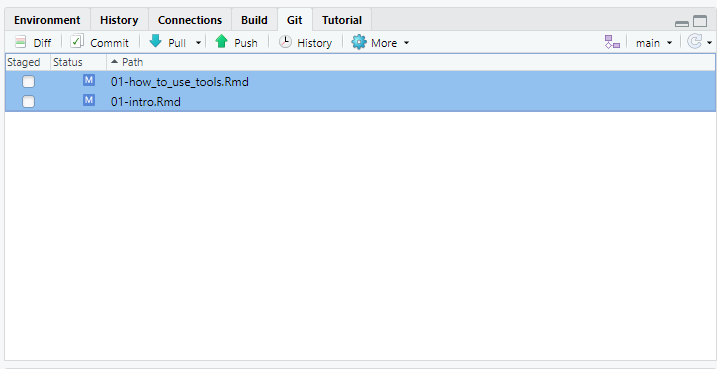
\includegraphics{01-how_to_use_tools_insertimage_1.png}

\hypertarget{tham-khux1ea3o}{%
\section{Tham khảo}\label{tham-khux1ea3o}}

\url{https://rstats.wtf/}

  \bibliography{book.bib,packages.bib}

\end{document}
